

\subsection{DVMS}

%\subsubsection{Overview.}
DVMS~\cite{quesnel:ispa2013,quesnel:cpe2012}
(Distributed Virtual Machine Scheduler) is a framework that schedule VMs
cooperatively and dynamically in large scale distributed
systems. It is deployed as a set of agents that are organized following a ring
topology and that cooperate with one another to guarantee that VM demands are satisfied during their executions. 
Concretely, when a node cannot guarantee the QoS for its hosted VMs or when it is
under-utilized, it starts an iterative scheduling procedure~(ISP) by querying
its neighbor to find a better placement ; it thus becomes the initiator of the ISP.
If the request cannot be satisfied by the neighbor, it is forwarded to the
following free one until the ISP succeeds. When a viable mapping has been
found, the leader (\ie the last peer that has taken part to the ISP) reconfigures 
the system by performing adequate VM migrations.
Such an approach allows each ISP to send requests only to a minimal number of
nodes and even though an ISP can reserve all nodes if the corresponding problem
is particularly hard to solve (guaranteeing thus that a solution will always be
found it it exits), experiments have shown that in most cases ISPs involve only
few nodes.  Moreover, the DVMS proposal allows several ISPs to occur
independently at the same moment throughout the infrastructure; in other words,
scheduling is performed on partitions of the system that are created
dynamically, which significantly improves the reactivity of the system.  To
prevent conflicts that could occur if several ISPs performed concurrent
operations on the same PMs or VMs, it should be noted that PMs are reserved for
exclusive use by a single ISP. 

An example involving three partitions is shown on Figure~\ref{fig:isp}; in
particular, we can see the growth of partition~1 between two steps. 
Explaining in details the notion of ``first out'' is beyond the scope of this article but readers can consider that the ``first out'' relation enables
to handle communications efficiently, as each node involved in a partition
can forward a request directly to the first node outside its partition~\cite{quesnel:cpe2012}.
\begin{figure}[h!]
  \centering
  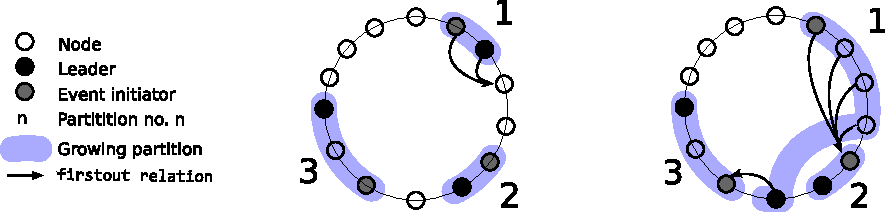
\includegraphics[width=0.9\linewidth]{Figures/resourceAcquisition-standard.pdf}
  \caption{Solving three problems simultaneously and independently with DVMS}%
\small{The ring has been matched on top of three sites}
  \label{fig:isp}%
\end{figure}

In addition to formally prove the correctness of DVMS, the first version of the prototype
has been validated at large scale (up to 80k VMs and 8k nodes by means of simulations and up to 4.7k VMs and 470 nodes by means of experiments on the Grid'5000
testbed~\cite{quesnel:ispa2013}).

As discussed earlier, one limitation of this approach is related to its ring topology that prevents to take into account the network topology. 
%\subsubsection{Limitations of The Ring}
%
%Even though  DVMS can be deployed across several sites, it performs better on a
%cluster.
%
%The reason is simple.
%
%The ring is built without taking account of the network  topology; 
In other words, if the ISP strategy enables to limit the size of one partition to a minimal number of nodes, these nodes are selected without considering 
the network conditions at the time the ISP starts; leading to inefficient situations where VM migrations occur between two nodes that are far from each other, 
which lasts longer than a migration between two close nodes. Obviously the ring can
be built in order to limit the distance between peers globally (\ie peers of
the same region/area would be grouped together as illustrated on Figure \ref{fig:isp}). However, in such a case at least two nodes of each group are directly connected to 
two far nodes. 
%
To sum up, the DVMS proposal lacks of a topology that can consider locality properties of a multi-sites infrastructure. 

\AL[CD/MB]{Can we add one sentence to make the transition to the next section: something for instance that explains that a hierarchy of rings will not tackle the aforementioned concern.}
% Autres limitations :
% -absence de tolérance aux pannes
% -peu d'événements gérés (surcharge d'un noeud)
% -ne prend pas en compte les liens entre VMS

\subsection{Overlay networks and locality}

Taking the locality into account in the construction of overlay networks was
initially proposed in the Pastry overlay network~\cite{pastry}. In order to
reduce the latency of the routing process, each node is given the opportunity to
choose the closest nodes to fill its routing table. Learning the existence of
new nodes relies on periodic exchange of the references of nodes known by nodes.


Le m?me concept a ?t? propos? dans les r?seaux logiques non structur?s afin de
permettre ? chaque n\oe ud de d?couvrir des n\oe uds du syst?mes les plus
\emph{proches}. La notion de proximit? peut recouvrir toute m?trique transitive
entre deux n\oe uds, en particulier le temps de latence entre les n\oe
uds~\cite{refquivabienmarindoittrouver}.

Le protocole Vivaldi~\cite{dabek:2001:sigcomm04}, sur lequel notre r?seau logique est fond?,
a une approche particuli?re. En effet, il fournit ? chaque n\oe ud des
coordonn?es dans un espace multi-dimensionnel refl?tant sa position dans le
r?seau physique. Initialement, chaque n\oe ud prend une position al?atoire de
l'espace, et choisit un petit sous-ensemble de n\oe uds. Puis, il se rapproche
dans l'espace, des n\oe uds avec lesquels il a une faible latence et s'?loigne
dans le cas inverse. Vivaldi ne permet donc pas de conna?tre les n\oe uds qui
lui sont proches dans le r?seau, mais de les reconna?tre via leurs coordonn?es.

Les approches pr?c?dentes maintiennent constamment la connaissance des n\oe udes
proches afin de fournir le meilleur n\oe ud possible, au co?t de communications
p?riodiques (ind?pendamment de la quantit? de requ?tes effectives.) Notre
approche se distingue par une approche paresseuse consistant ? rechercher des
n\oe uds proches (en s'appuyant sur les coordonn?es Vivaldi) lors des requ?tes,
adaptant ainsi la qualit? de la r?ponse ? la fr?quence des requ?tes.

